\documentclass[12pt]{report}
\usepackage[margin=1in]{geometry}
\usepackage{setspace} % for single/doublespacing commands
\usepackage{graphicx} % including graphics
\usepackage{sectsty} % sexy section headings
\usepackage{pdfpages} % including multipage pdfs
\usepackage[export]{adjustbox} % for graphic frames and center
\usepackage{siunitx}
\usepackage[numbered]{matlab-prettifier} % including matlab w/ syntax highlighting
\usepackage[T1]{fontenc} % prettier matlab font
\usepackage{xfrac} % more legible inline fractions (\sfrac)
\usepackage{lmodern} % font package for above
\usepackage{multicol} % multiple columns
\usepackage[justification=centering]{caption} % figure captions (force centering)
\usepackage{amsmath} % more math symbols and shit
\usepackage{enumitem} % add arguments for enumerate to change style
\usepackage[list=true]{subcaption} % subfigures with list of figure support
\usepackage{multirow}
\usepackage{mathtools}
\usepackage{booktabs}
\usepackage{color}
\usepackage{ulem}
\usepackage{blindtext}
\usepackage[numbers]{natbib}
\usepackage{contour}
\usepackage{tabularx}
\usepackage{circuitikz} % drawing fancy shit
\usepackage{cancel} % arrow and cross math cancel symbol
\usepackage{lineno}
\usepackage{framed}
\usepackage{amssymb} % special math symbols
\usepackage{listings}
\usepackage{array}
\usepackage{BOONDOX-cal} % fancy mathtype script
\usepackage{fancyhdr}
\usepackage{flowchart}
\usepackage{color, colortbl}
\usepackage{tocloft}
\usepackage{url}
\usepackage{etoolbox}

\setcounter{secnumdepth}{5}
\renewcommand{\bibname}{References}
\sisetup{output-exponent-marker=\ensuremath{\mathrm{e}}}
\newcommand{\PreserveBackslash}[1]{\let\temp=\\#1\let\\=\temp}
\newcolumntype{C}[1]{>{\PreserveBackslash\centering}p{#1}}
\newcolumntype{R}[1]{>{\PreserveBackslash\raggedleft}p{#1}}
\newcolumntype{L}[1]{>{\PreserveBackslash\raggedright}p{#1}}
\lstMakeShortInline[style=Matlab-editor]| % matlab inline escape character
\graphicspath{{images/}}
\renewcommand\thesection{\arabic{section}}
\renewcommand\labelitemi{---}
\lstset{numberstyle=\ttfamily\small\color{gray}}
\renewcommand\linenumberfont{\ttfamily\small\color{gray}}
\setlength\linenumbersep{6mm}
% \hbadness=99999  % or any number >=10000
\apptocmd{\sloppy}{\hbadness 10000\relax}{}{}
\usetikzlibrary{arrows,calc,patterns,angles,quotes}
\usetikzlibrary{shapes.geometric}
\usetikzlibrary{decorations.pathmorphing,decorations.pathreplacing} % for snakes!
\usetikzlibrary{positioning, circuits.logic.US}
% Define block styles
\tikzstyle{decision} = [diamond, draw, fill=white!20,
    text width=5em, text badly centered, node distance=3.5cm, inner sep=0pt]
\tikzstyle{term} = [rectangle, draw, fill=white!20,
    text width=5em, text centered, rounded corners, minimum height=2em]
\tikzstyle{block} = [rectangle, draw, fill=white!20,
    text width=5em, text centered, minimum height=4em]
\tikzstyle{line} = [draw, -latex']
\tikzstyle{cloud} = [draw, ellipse,fill=white!20, node distance=3cm,
    minimum height=2em]
\tikzstyle{data} = [trapezium,trapezium left angle=70,
    trapezium right angle=-70,draw, minimum height=1cm]
\tikzstyle{proc} = [draw, predproc, align=center,
    minimum width=4em, minimum height=1cm]
\setlength{\cftbeforetoctitleskip}{-2em}
\newcommand{\Lag}{\mathcal{L}} % lagrangian L
\begin{document}
\normalem
\begin{titlepage}
\flushleft
\doublespacing
\Large
\textsc{Test Document} \\
\normalsize
Trey Dufrene, Zack Johnson, David Orcutt, Alan Wallingford, Ryan Warner
\vfill
\center
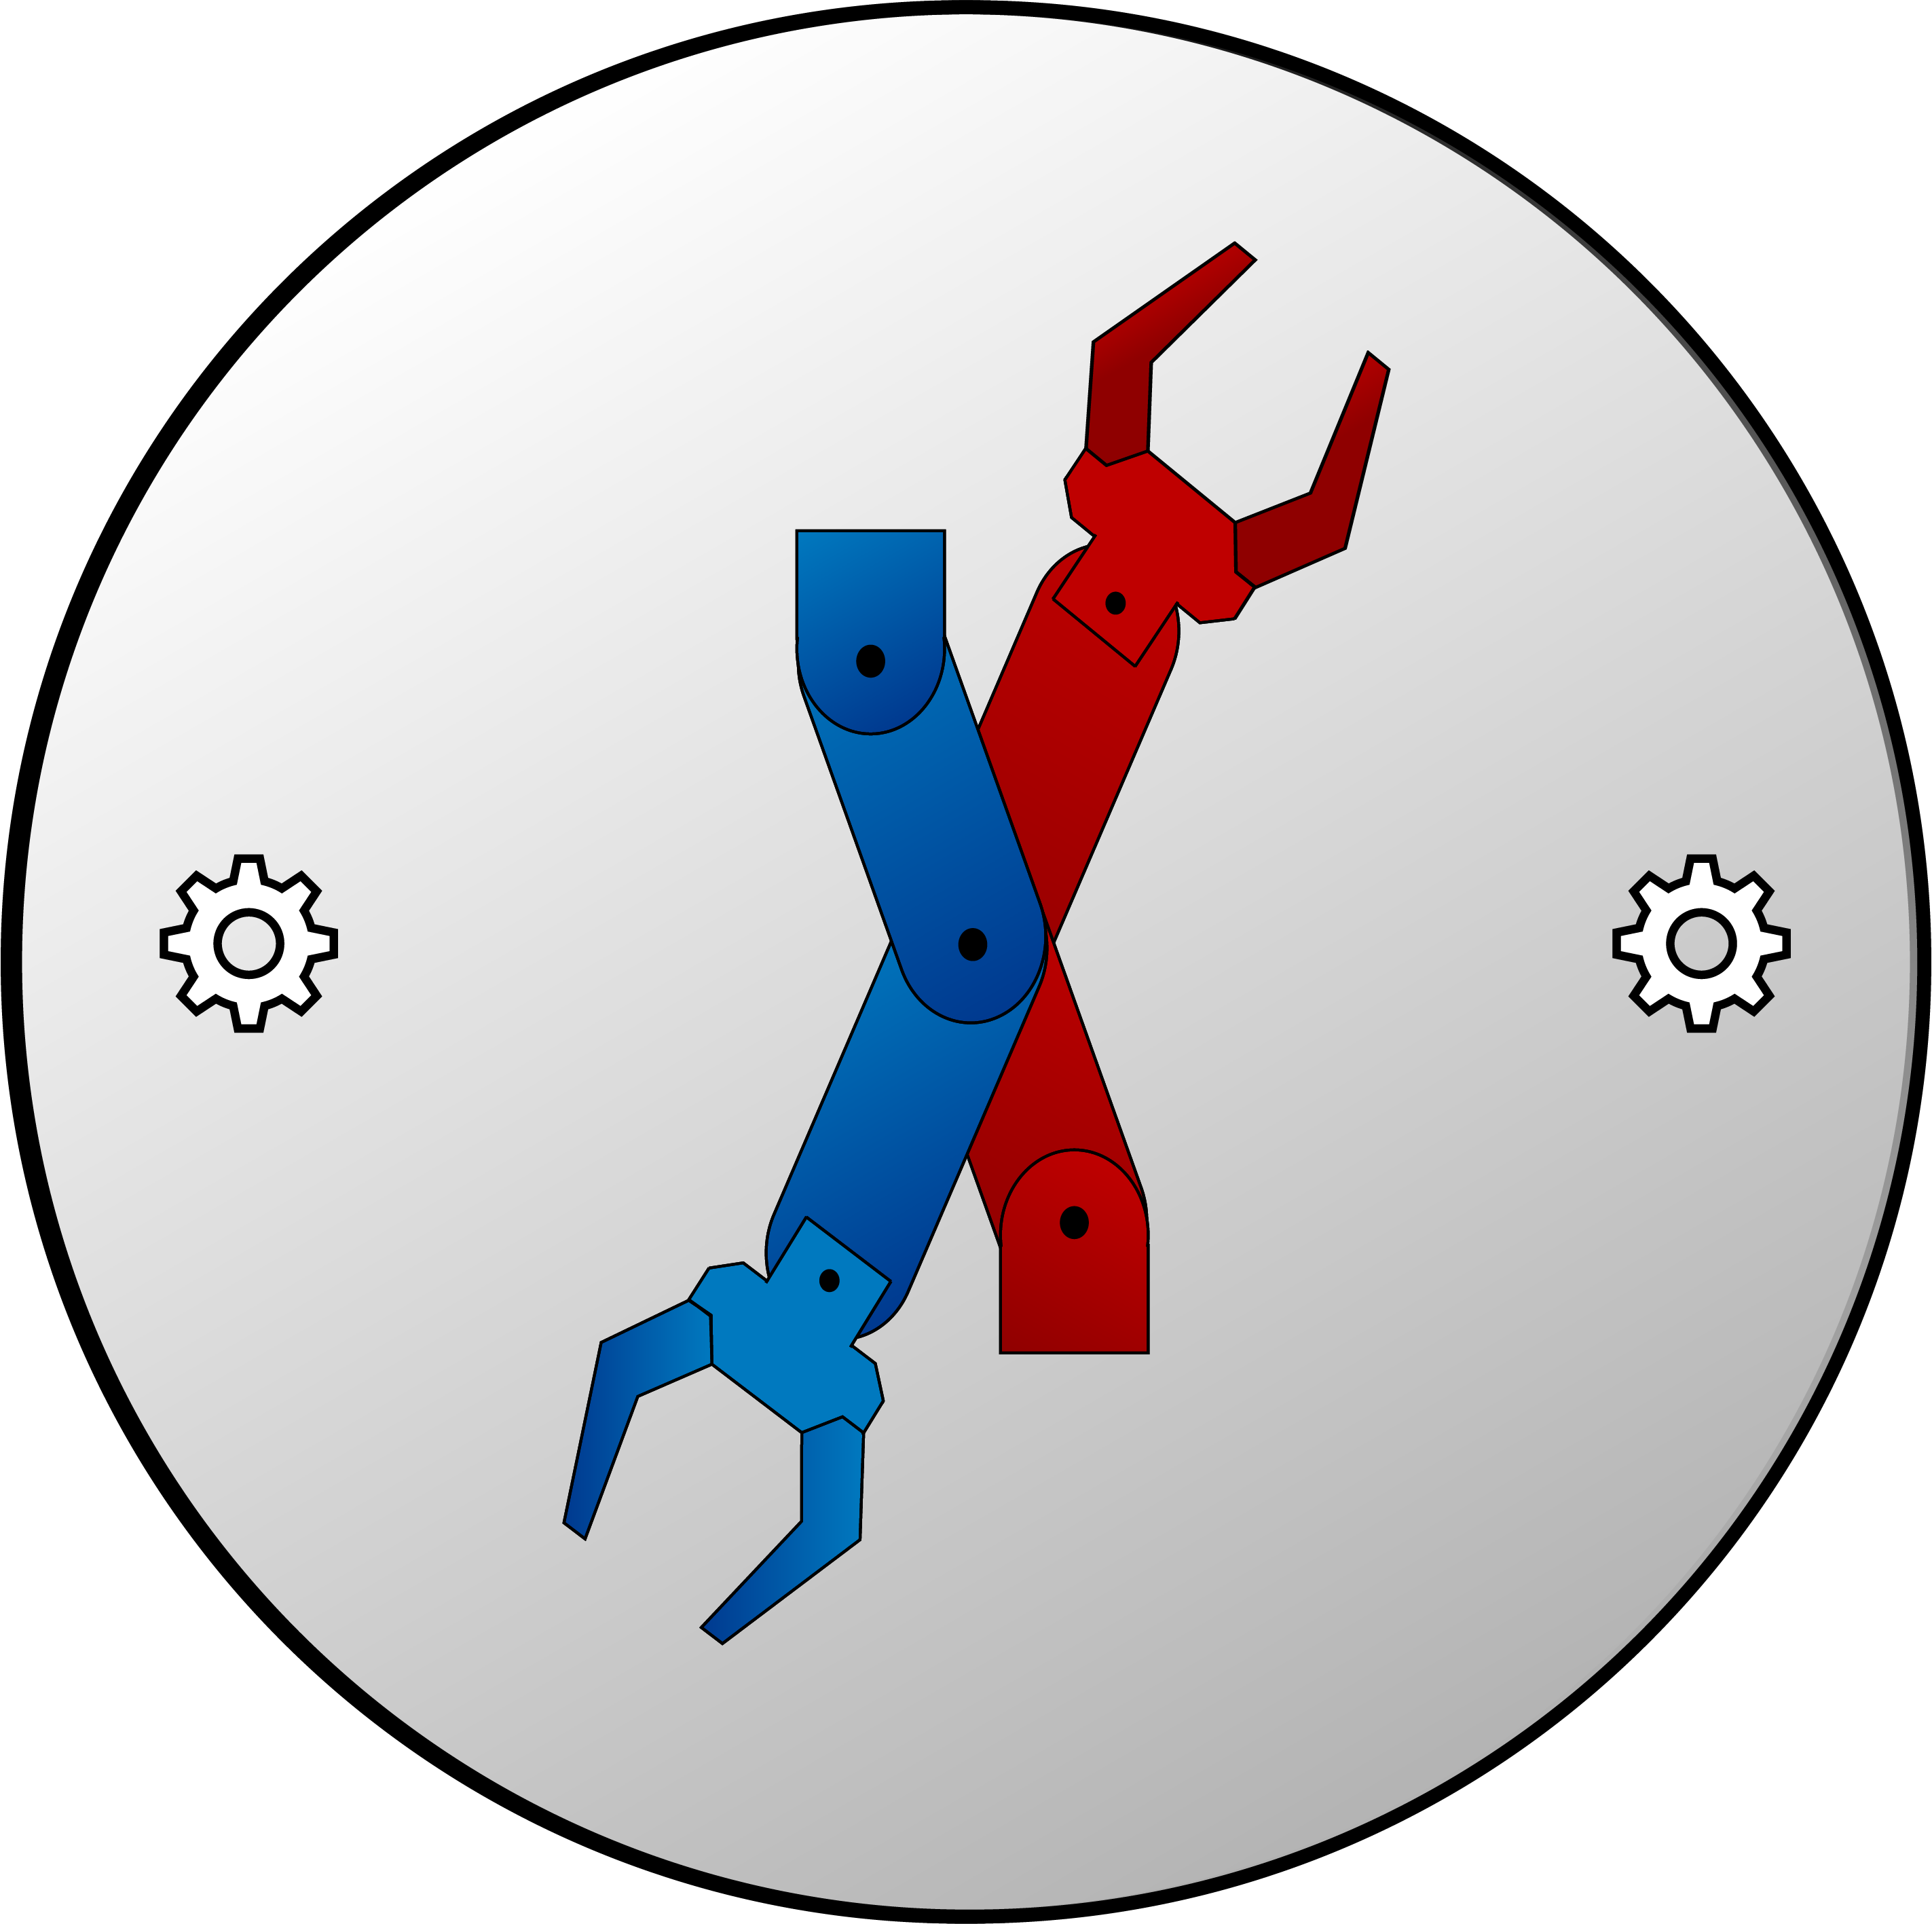
\includegraphics[width=.45\textwidth]{logo}
\vfill
\flushleft
ME 407 \\
Preliminary Design of Robotic Systems \\
Embry-Riddle Aeronautical University \\
\vspace{2ex}
\begin{minipage}[c]{.5\textwidth}
\flushleft

\includegraphics[width=.95\textwidth]{erau}
\end{minipage}%
\begin{minipage}[c]{.5\textwidth}
\flushright

\includegraphics[width=.8\textwidth]{text}
\end{minipage}
\end{titlepage}

\pagenumbering{roman}
% \begin{abstract}
  % Wordy words
% \end{abstract}
{\tableofcontents\let\clearpage\relax\listoffigures\let\clearpage\relax\listoftables}
\clearpage
\newpage

% \section*{List Of Acronyms and Abbreviations}

% \begin{tabular}{rl}
%   $G$~:&Center of gravity of the bar \\
%   $\ell_0$~:& Spring unstretched length  \\
%   $\delta$~:& Spring deflection \\
%   $k$~:& Spring constant \\
%   $h_{b}$~:& Distance to bar ($G$) from datum \\
%   $F_s$~:& Force onto bar due to spring\\
%   $A_{n}$~:& Pin reaction in $\theta$ direction\\
%   $A_{t}$~:& Pin reaction in tangential direction \\
%   $\vec{v}_G$~:& Velocity of bar center of gravity\\
%   $\ddot{\theta}$~:& Angular velocity of spring \\
%   $\ddot{\phi}$~:& Angular velocity of bar\\
%   $\ddot{\ell}_s$~:& Radial acceleration of spring \\
% \end{tabular}
% \normalsize
% \flushleft
% \singlespacing
% \newpage

\pagenumbering{arabic}
\onehalfspacing
\section{Introduction}
The terminator T-2000 is a science-fiction spectacle of a manipulator-- until you see the price. Channeling the inspiration many high school students may have for robotics, MEIOSIS robotics aims to provide an affordable manipulator to educators and enthusiasts. MEIOSIS uses primarily 3-D printed components and easily accessible materials. Among these materials are a Raspberry PI , smart servos and metal tubing. These features create an open-source manipulator accessible to the public to further robotics education.
\section{Physical System Overview}
\emph{Figure \ref{fig:overall}} shows the overall design for the manipulator. Much of the system’s physical design will be determined during the actual design of the manipulator, after the specifications stage. The figure below shows the basic overall conceptual design of the manipulator, having all six rotational joints, the latter three of which being in a spherical wrist configuration.

\begin{figure}[htp]
  \centering
  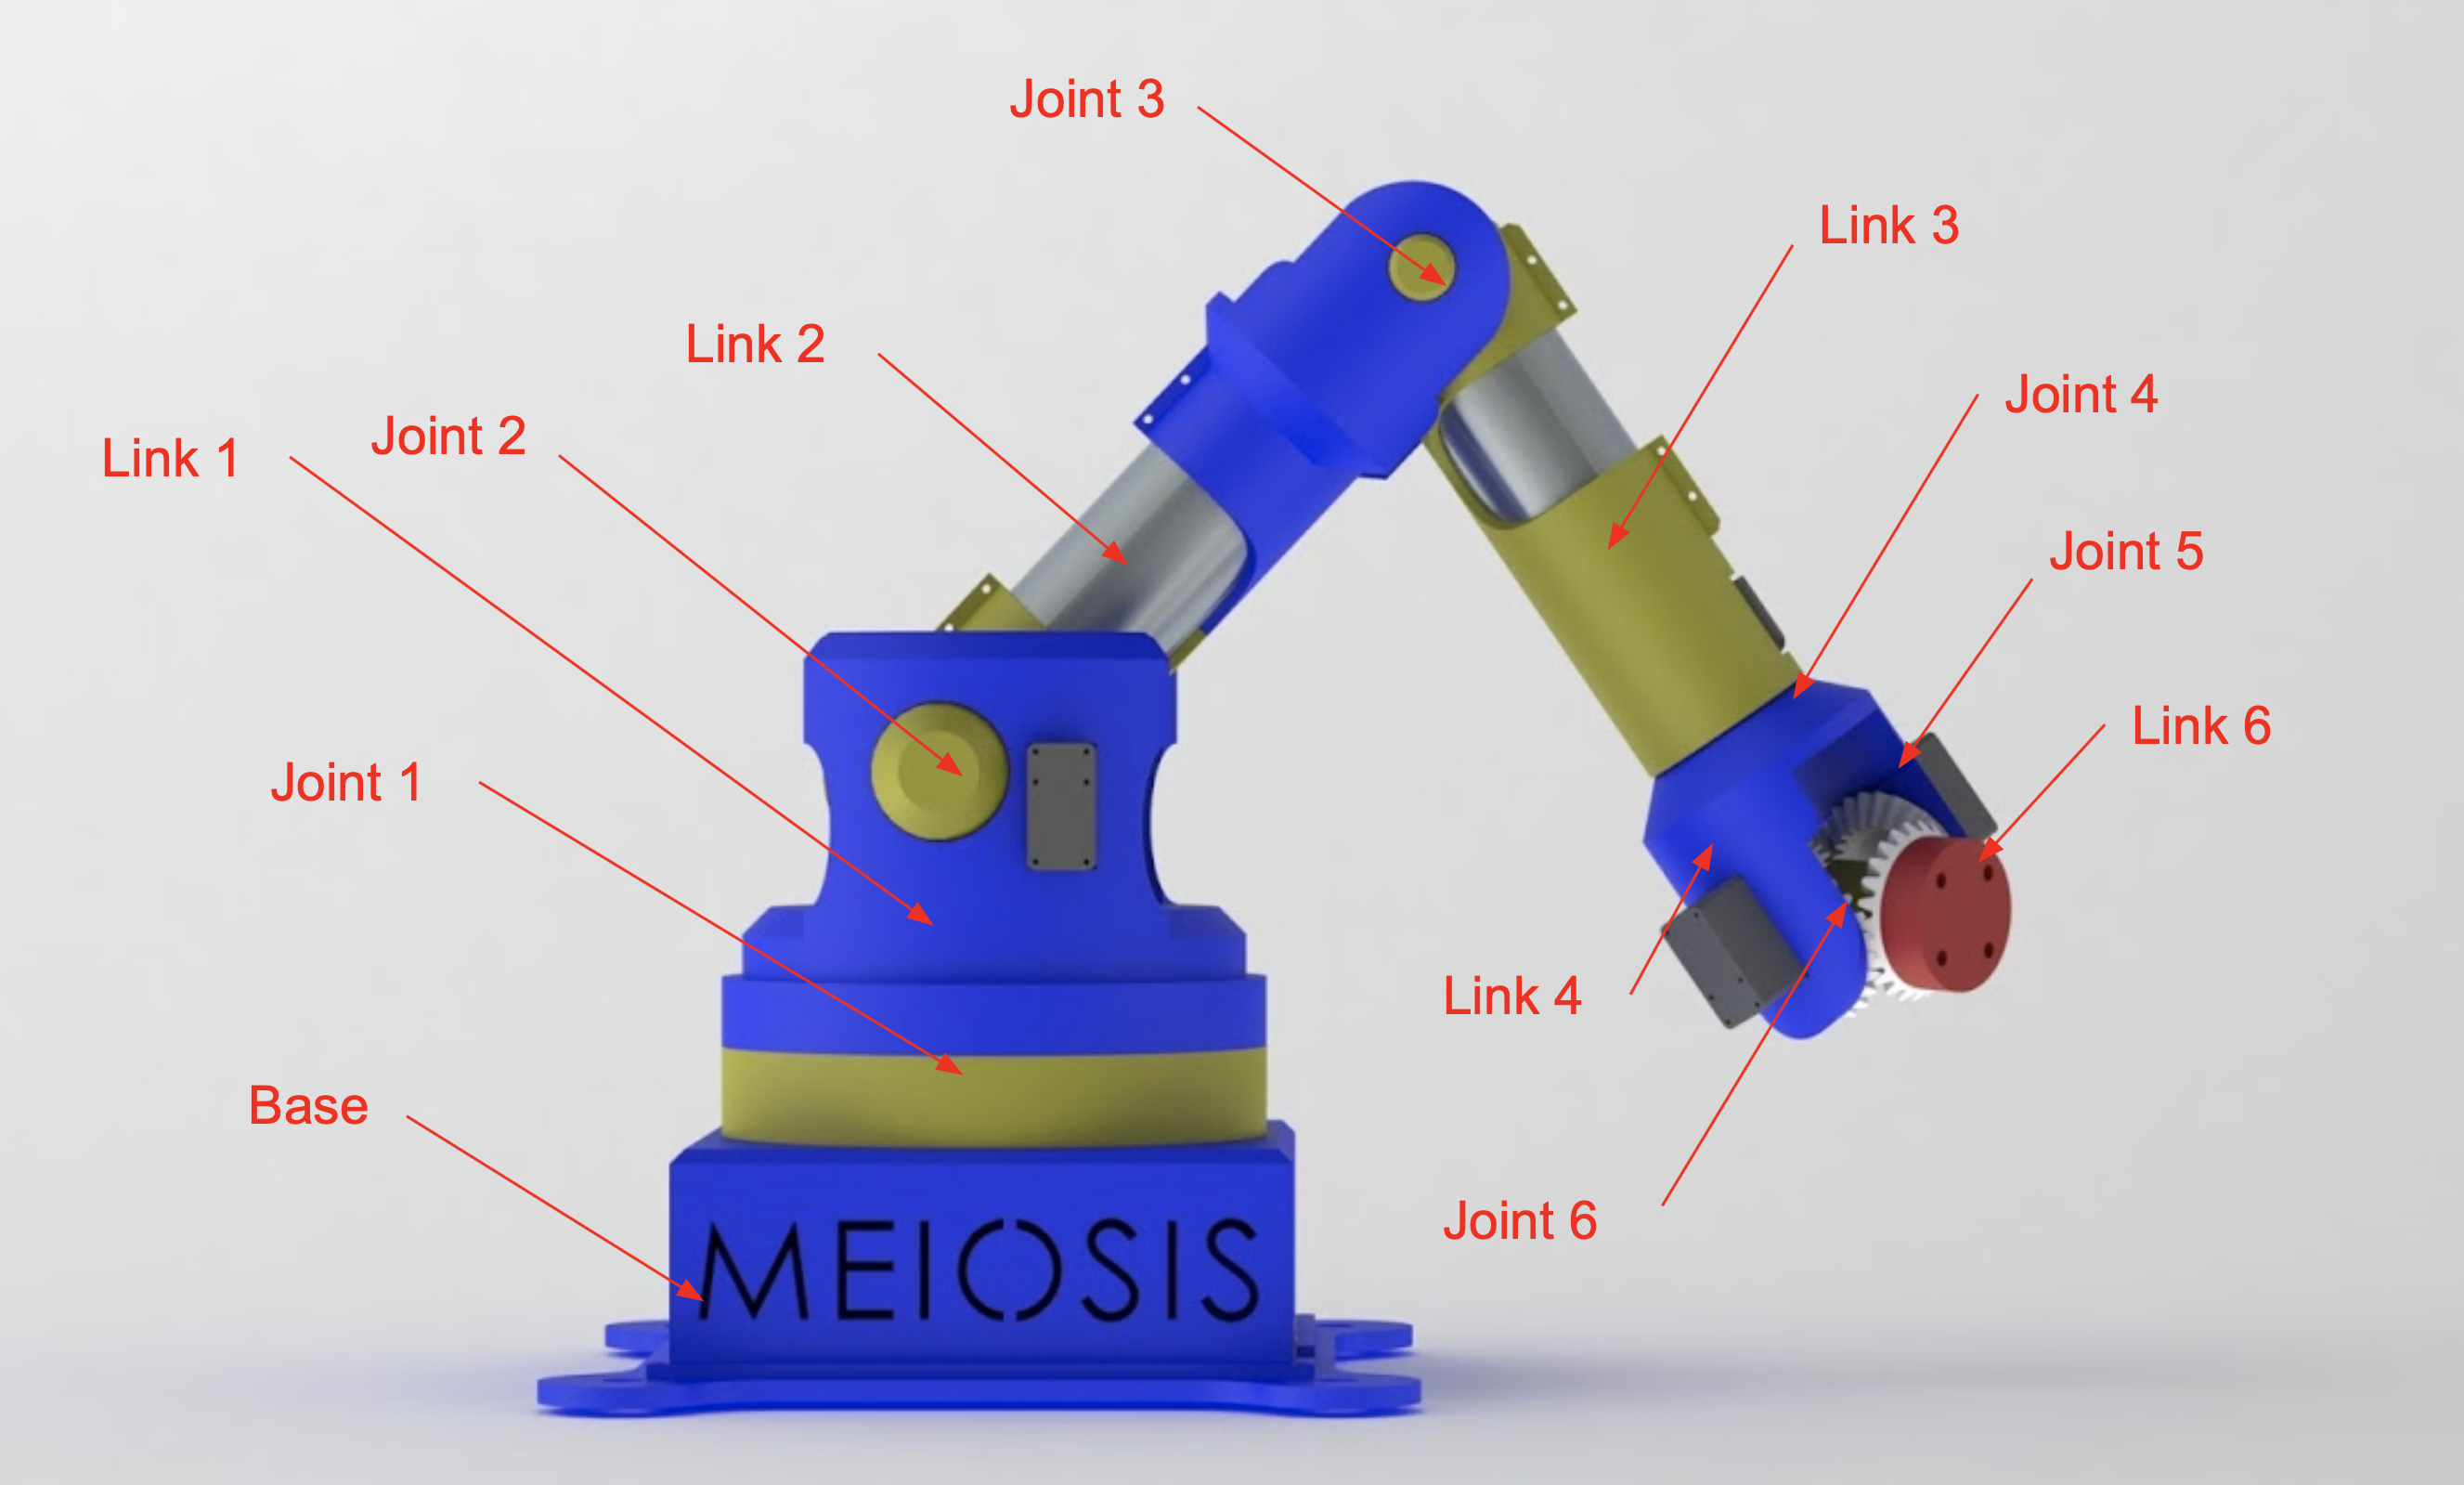
\includegraphics[frame, width=.75\textwidth]{overall_render}
  \caption{Overall System Conceptual Design }
  \label{fig:overall}
\end{figure}

The colored links in \emph{Figure \ref{fig:overall}} distinguish the different joints and links of the manipulator. The overall reach of the robot will be 500 mm. This length was chosen to decrease material cost and weight while still satisfying requirement 2.1.2 and 2.1.5, allowing the manipulating to pick and place objects to perform basic tasks. The base of the robot will be made to contain the Raspberry Pi and other electrical components.
\newpage
\subsection{Base}
The base of the manipulator will house several of the electronic components, such as the computational sytem, power supply, and motor controller. A cross section of the base can be seen in \emph{Figure \ref{fig:base}}.
\begin{figure}[htp]
  \centering
  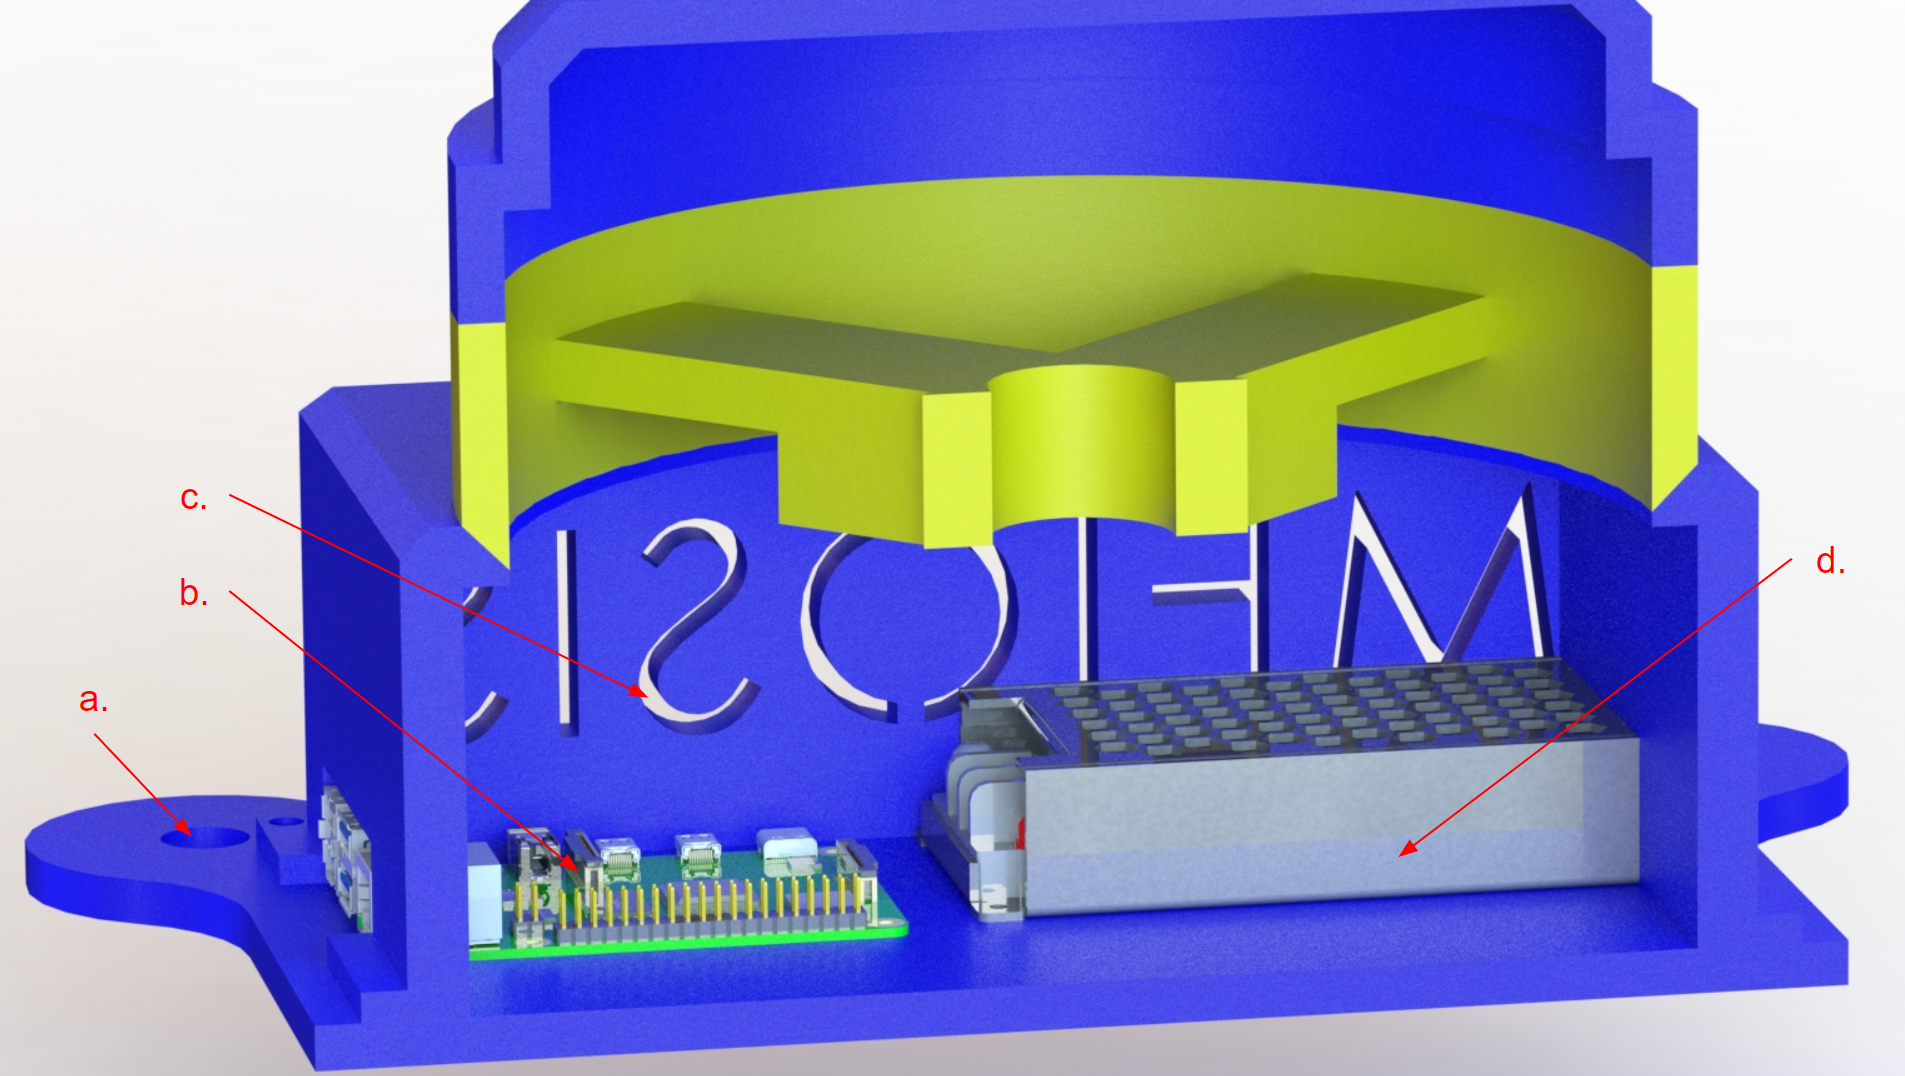
\includegraphics[frame, width=.75\textwidth]{base_callouts}
  \caption{Manipulator Base with Callouts}
  \label{fig:base}
\end{figure}

From \emph{Figure \ref{fig:base}},
\begin{enumerate}[label=\alph*.]
  \item \emph{Base Supports:}
  The base supports are located at each corner of the base and will allow the base of the manipulator to be securely attached to a variety of surfaces with either standard bolt/fastener hardware or suction cups.
  \item \emph{Computational System:}
  The computational system will consist of a Raspberry Pi; the primary reason for this system being chosen is to fulfill the budget requirement, 2.1.1. The Raspberry Pi will perform the necessary computations for solving the kinematics of the manipulator and command the motors accordingly.
  \item \emph{Airflow Cutouts:}
  The side of the base will have cutouts to allow for the maximum amount of airflow to pass through; since the power supply is housed inside of the base as well as the computational system, the temperature must be regulated to prevent overheating.
  \item \emph{Power Supply:}
  The power supply will be housed in the base as well; this allows the system to be more accessible and therefore more modifiable, where the end-user can easily expand the system to fulfill their needs.
\end{enumerate}
\newpage
\subsection{Links}
\emph{Figure \ref{fig:link1}} shows a few of the key features of our design. Point a shows the connection point for the end effector. The dimensions are the standard used by the Sawyer manipulator. This will likely be adjusted depending on the desired end effector. Point b shows the differential gearbox that will be used in the wrist of the robot. This allows for saved space and weight. The manipulator will have aluminum tubing as support in the links (c) and will be attached to the 3D printed portion of the robot using clamp joints (d) which are tightened by screws.

\begin{figure}[htp]
  \centering
  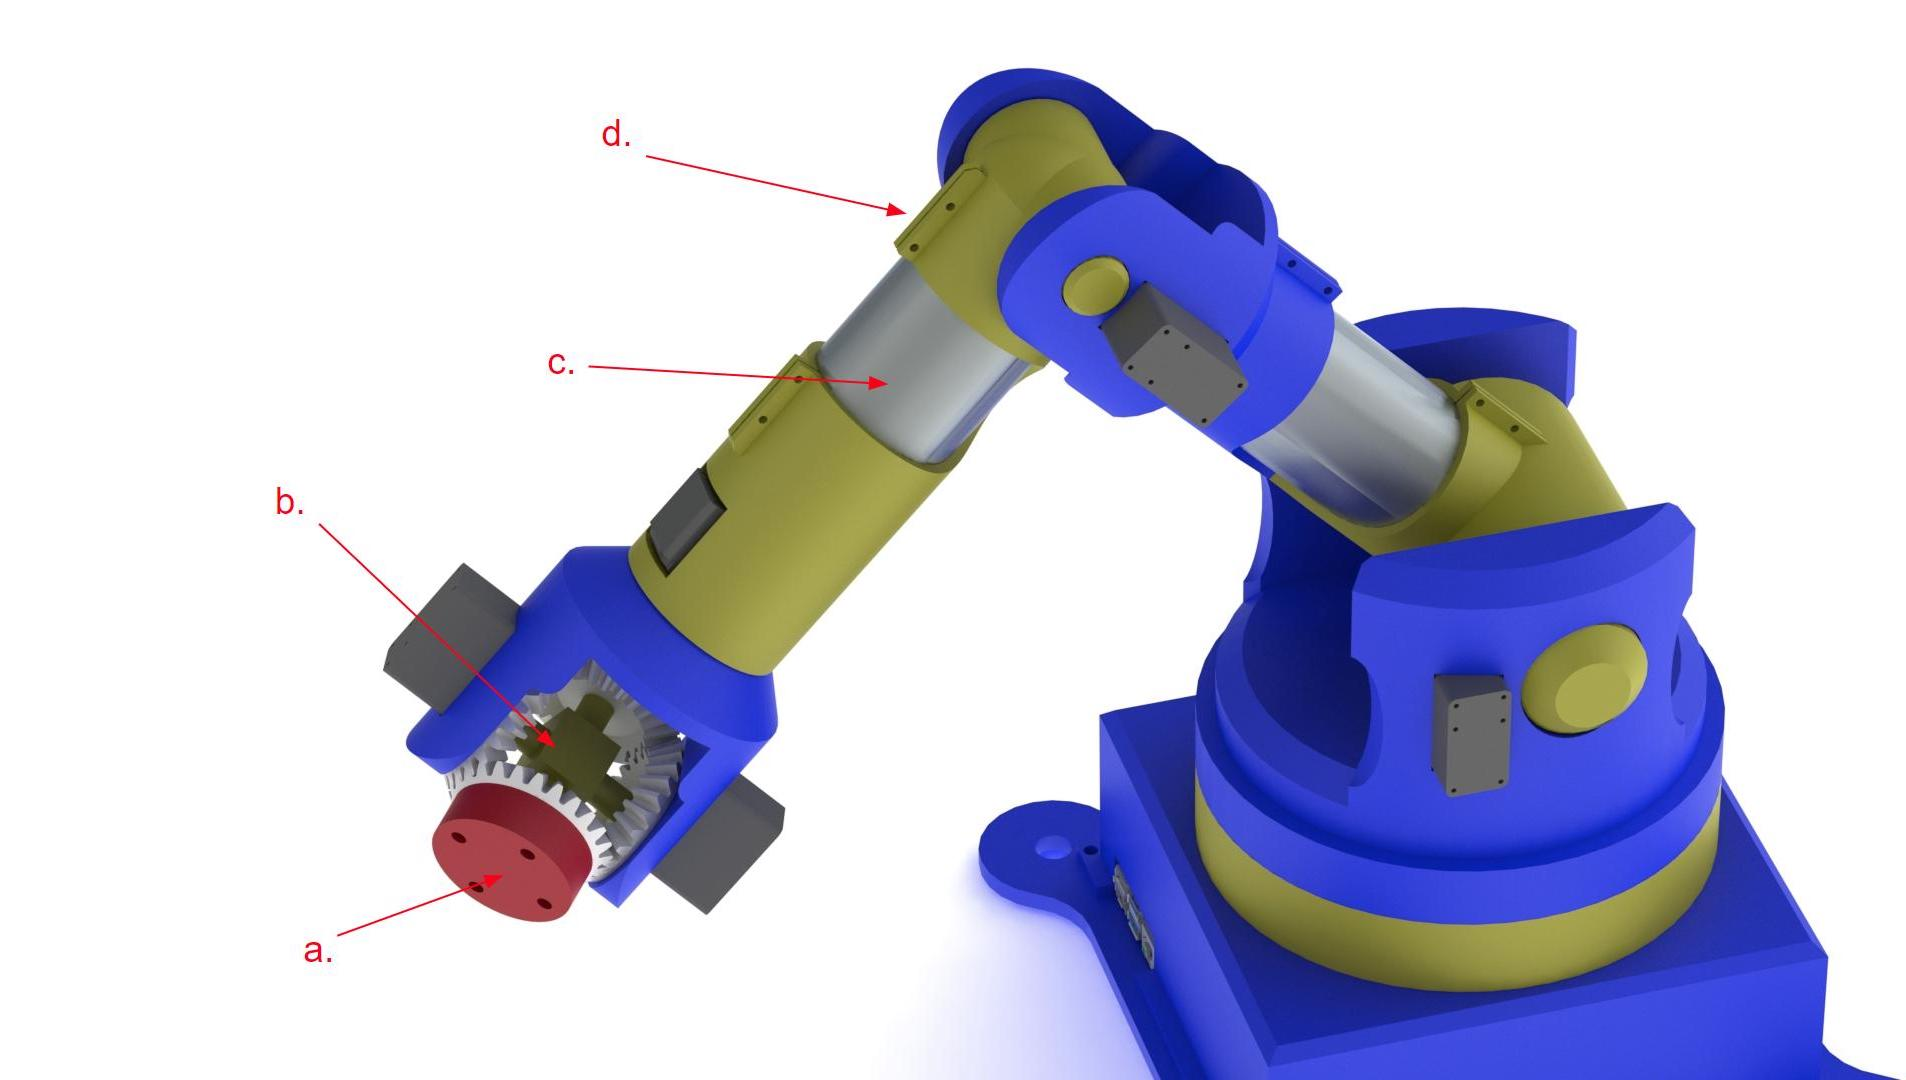
\includegraphics[frame,width=.75\textwidth]{link_callouts}
  \caption{Drawing Showing Key Features of Design}
  \label{fig:link1}
\end{figure}

\begin{figure}[htp]
  \centering
  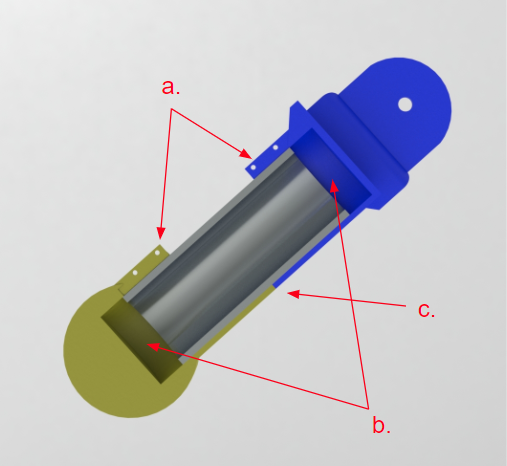
\includegraphics[frame,width=.5\textwidth]{link_cross_section}
  \caption{Drawing Showing Link Cross Section}
  \label{fig:link2}
\end{figure}
\newpage
\emph{Figure \ref{fig:link2}} shows the cross section for the design of the links. This features two clamps that hold the aluminum bar in place (a) and allows for gaps between the aluminum tube and the 3D printed part. This allows for imprecise measurements in the aluminum tube that could be caused by the end user. The aluminum tube will be cut shorter than the actual required distance which will result in gaps between the tubing and the part (b). The proper distance will be achieved by the 3D printed parts lining up at point c.

\section{System Functions}
The system consists of two primary categories, the electrical and software systems. The electrical subsystem includes the wiring and hardware computational components, power system, actuators with drivers, and sensors. The software subsystem includes the algorithm flowchart for the computational system.
\subsection{Electrical}
\begin{figure}[htp]
  \centering
  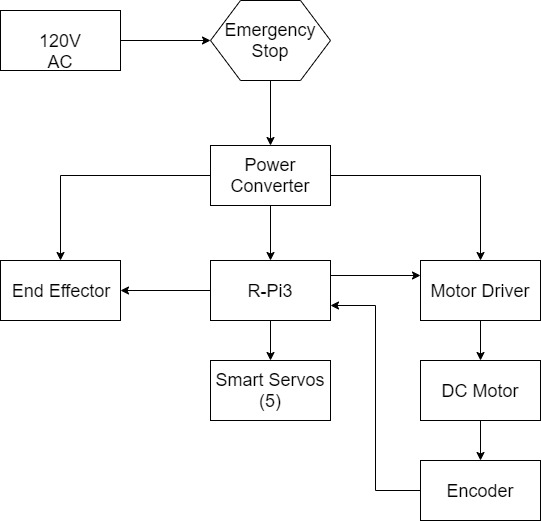
\includegraphics[width=.55\textwidth]{eblock}
  \caption{Electrical System Block Diagram}
  \label{fig:eblock}
\end{figure}

\emph{Figure \ref{fig:eblock}} shows that the electrical systems of the manipulator will be relatively simple, with power being supplied by the standard 120V AC available from wall outlets. A power converter will be used to adapt the AC voltage to the required voltages for each component. To control the system, a Raspberry Pi will perform the necessary calculations for motor control (described below in software). It will then send these signals to the DC motor driver and the five smart servos. The smart servos have an on-board controller, so no feedback will be necessary. However, the first rotational joint between the base and the first link will be actuated by a DC motor with an encoder to minimize cost.

\subsection{Software}
\begin{figure}[ht]
  \centering
  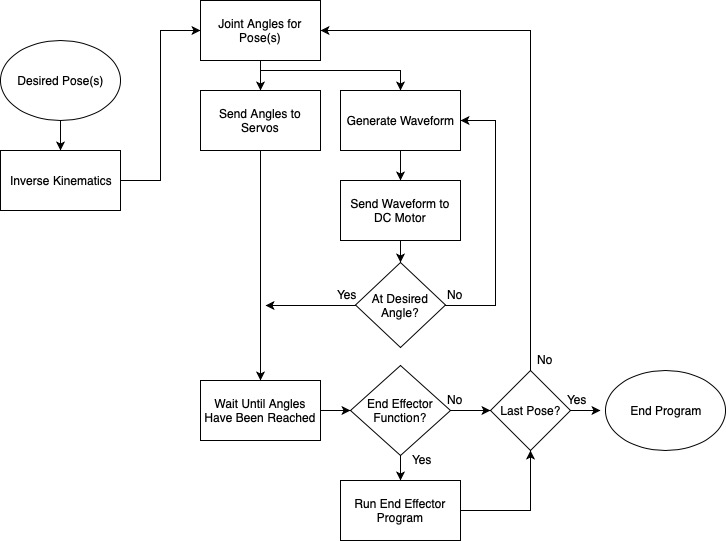
\includegraphics[width=.85\textwidth]{sblock}
  \caption{Software Flowchart}
  \label{fig:sblock}
\end{figure}

Similar to the electrical system, the software required for the system to function is not complex. \emph{Figure \ref{fig:sblock}} shows how the software will receive the desired pose or poses that the user would like the manipulator to reach and calculate the inverse kinematics to find the necessary joint angles to reach the pose. The waveforms/desired angles will be sent to the respective drivers/motors, and if a motor requires feedback to reach the correct position, positional information will be sent back to the computer so that the proper waveform will be sent to the respective motor at all times. When the motors have reached their desired positions, the controller will run the end effector function if it is called. The system will then check to see if there are any more poses to reach and either repeat the motor control section given the desired angles of the new pose or end program if the last pose has been reached.

\section{Parts List and Manufacturing}
Our costs are estimated from all specific components we invision requiring with a factor of safety. The 20\% factor of safety is the sum of 20\% of the cost for each item listed in Table 4.1 and is intended to account for shipping, taxes, and replacement/additional parts. Including this factor of safety, we satisfy requirement 2.1.2 with a predicted budget of \$586.80.

\begin{table}[htp]
  \center
  \caption{Predicted List of Parts}
  \label{table:costs}
  \begin{tabular}{C{3.5cm}cc|cc}
  \textbf{Part} & \textbf{Unit Cost (USD)} & \textbf{Qty} & \textbf{Cost (USD)} & \textbf{Source} \\ \hline
  2kg PLA & 32 & 1 & 32 & Amazon \\
  Smart Servo & 140 & 2 & 280 & Trossen Robotics \\
  Lower Torque Smart Servo (6 pack) & 225 & 1 & 225 & Trossen Robotics \\
  DC Motor w/ Encoder & 30 & 1 & 30 & Robot Shop \\
  Power Supply & 16 & 1 & 16 & Compt. Dist. Inc. \\
  Rasberry Pi 3 & 35 & 1 & 35 & Adafruit \\
  3 Pin Cables & 9 & 1 & 9 & Amazon \\
  4 Pin Cables & 13 & 1 & 13 & Amazon \\
  Gripper & 25 & 1 & 25 & Trossen Robotics \\
  Factor of Safety (20\%) & & & 133 & \\
  & & \textbf{Total} & 798 & \\
  \end{tabular}
\end{table}

Our motor costs are approximated from three motor types. For use in joint one is one stepper motor \cite{robotis}. It should experience minimal torque from gravity acting on the other links and does not require a continuous voltage to maintain position. The built-in encoder provides feedback for accurate motion and limiting the rotation to 2$\pi$ radians. For use in joints two and three are two smart servos with holding torque of 1.6N$\cdot$m. These feature a built in PD control, which means no overshooting, that can be precise to 0.29\(^{\circ}\) with tuning \cite{matterhackers}. So long as the links, servos, and payload after the base do not exceed 0.65kg acting through the horizontally outstretched arm’s centroid, 250mm from the base, the torque is sufficient. Although the servos are continuous rotation, joints two and three are not free to rotate \(360^{\circ}\). Finally, for the spherical wrist are three lower cost, lower torque smart servos, which also have PD control \cite{rev}. The gripper will also be actuated with one of these servos.

Since each motor has the same voltage requirement of 12V and our manipulator is powered by 120V AC, we also account for the cost of a power supply. The power and communication buses are handled by four pin wires for the smart servos and three pin wires for the lower-cost smart servos. 2kg of PLA filament allows all components of the manipulator to be 3D printed with 100\% infill, making it an overestimate. With a 20\% factor of safety to account for shipping, taxes, and unexpected part purchases, we are under our team budget of \$800 and design budget of \$1000.
\definecolor{Gray}{gray}{0.5}

\begin{table}[htp]
  \center
  \caption{Gantt Chart}
  \label{table:gantt}
\begin{tabular}{C{2.9cm}|cccccccccccccccccc}
& \multicolumn{18}{c}{ Class Work Session } \\
Software \small & 1 & 2 & 3 & 4 & 5 & 6 & 7 & 8 & 9 & 10 & 11 & 12 & 13 & 14 & 15 & 16 & 17 & 18 \\\hline\normalsize
\textbf{Kinematics} & \cellcolor{Gray} & \cellcolor{Gray} & \cellcolor{Gray} & \cellcolor{Gray} & \cellcolor{Gray} & & & & & & & & & & & & & \\
Microcontroller Compatability & \cellcolor{Gray} & \cellcolor{Gray} & & & & & \cellcolor{Gray} & \cellcolor{Gray} & & & & & & & & & & \\
Motor Actuation & & \cellcolor{Gray} & \cellcolor{Gray} & \cellcolor{Gray} & \cellcolor{Gray} & \cellcolor{Gray} & \cellcolor{Gray} & \cellcolor{Gray} & & & & & & & & \cellcolor{Gray} & \cellcolor{Gray} & \cellcolor{Gray} \\\hline
\textbf{Motors} & & & & & & & & & & & & & & & & & & \\\hline
Model & & & & & & & & & \cellcolor{Gray} & \cellcolor{Gray} & \cellcolor{Gray} & \cellcolor{Gray} & \cellcolor{Gray} & \cellcolor{Gray} & & & & \\
Calibration & & & & & & & & & & & & & & & & \cellcolor{Gray} & \cellcolor{Gray} & \cellcolor{Gray} \\
Interfacing & & & & & & & & & & & & & \cellcolor{Gray} & \cellcolor{Gray} & \cellcolor{Gray} & \cellcolor{Gray} & & \\
\textbf{Links} & & & & & & & & & & & & & & & & & & \\\hline
Model & & & & \cellcolor{Gray} & \cellcolor{Gray} & \cellcolor{Gray} & \cellcolor{Gray} & \cellcolor{Gray} & \cellcolor{Gray} & & & & & & & & & \\
Print & & & & & & & & \cellcolor{Gray} & \cellcolor{Gray} & \cellcolor{Gray} & \cellcolor{Gray} & \cellcolor{Gray} & & & & & & \\
\textbf{Wiring} & & & & & & & & & & & & & & & & & & \\\hline
Bus Testing & & \cellcolor{Gray} & \cellcolor{Gray} & \cellcolor{Gray} & & & & & & & & & & & & & & \\
Mapping & & & & & & & & & \cellcolor{Gray} & \cellcolor{Gray} & \cellcolor{Gray} & \cellcolor{Gray} & \cellcolor{Gray} & & & & & \\
Implementation & & & & & & & & & & & & & & \cellcolor{Gray} & \cellcolor{Gray} & \cellcolor{Gray} & \cellcolor{Gray} & \cellcolor{Gray} \\
\textbf{Manipulator} & & & & & & & & & & & & & & & & & & \\\hline
Link Fitting & & & & & & & & & & & & \cellcolor{Gray} & \cellcolor{Gray} & \cellcolor{Gray} & \cellcolor{Gray} & & & \\
Calibration & & & & & & & & & & & & & & & & \cellcolor{Gray} & \cellcolor{Gray} & \cellcolor{Gray} \\
Gripper Interchangability & & & & & & & & & & & & & & \cellcolor{Gray} & \cellcolor{Gray} & & & \\
\end{tabular}
\end{table}


\emph{Table \ref{table:gantt}} shows approximately half of our time for Fall semester will be used modeling the manipulator’s kinematics, motor dynamics, and physical links with the second half dedicated to interfacing parts, wiring, and testing components. Nonetheless, the manipulator should have a functional guise by the semester’s end, however, we anticipate our design will require further iterations before it satisfies all our requirements. We do not account for a refined control interface usable by novice robotics students, rather functional simulations and programing for the manipulator.

\section{Decision Matrices}
The design for the end effector attachment varied across each of the team member’s original conceptual designs, therefore a decision matrix was constructed in order to objectively decide on the design chosen for the attachment style.

\begin{table}[htp]
  \center
  \caption{End Effector Attachment Design Decision Matrix}
  \label{table:ee}
\begin{tabular}{C{3.5cm}|cccc}
\textbf{EE Attachment} & \textbf{Ease of Use} & \textbf{Manufacturability} & \textbf{Durability} & Total \\
Weighting & 3.6 & 5 & 7 & \\\hline
Screw Connections & 6.8 & 8.8 & 9.8 & \textbf{137.08} \\
Snap Fit Joint & 8.6 & 5 & 2.2 & 71.36 \\
Threaded End Effector & 6.3 & 5.4 & 7.3 & 100.78 \\
\end{tabular}
\end{table}

As shown in \emph{Table \ref{table:ee}}, the design that is the optimal combination of  ease of use, the most manufacturable, and the most durable is the screw connections design.

\begin{table}[htp]
  \center
  \caption{Material Choice Decision Matrix}
  \label{table:mat}
\small\begin{tabular}{c|cccccc}
\textbf{Material} & \textbf{Cost} & \textbf{Weight} & \textbf{Accessibility} & \textbf{Manufacturability} & \textbf{Durability} & Total \\\normalsize
Weighting & 9.2 & 6.6 & 8 & 6.4 & 5.4 & \\\hline
3D Printed & 8 & 9 & 8 & 9.4 & 5 & 284.16 \\
Aluminum & 4 & 5.8 & 5.8 & 6.6 & 9.2 & 213.4 \\
Combination & 8 & 7.8 & 7 & 9 & 9.2 & \textbf{288.36} \\
\end{tabular}
\end{table}
As seen in \emph{Table \ref{table:mat}}, the primary material chosen to create the manipulator is PLA / 3D printed material, this is due to its low cost and weight, accessibility and manufacturability; additionally, by using primarily 3D printed parts, the end-user’s cost is potentially lower and their ability to modify parts if desired is much easier.

\begin{table}[htp]
  \center
  \caption{Computing Choice Decision Matrix}
  \label{table:comp}
\begin{tabular}{c|ccccc}
\textbf{Computing System} & \textbf{Cost} & \textbf{Capabilities} & \textbf{Ease of Use} & \textbf{Independance} & Total \\
Weights & 10 & 4.2 & 7.6 & 4.2 & \\ \hline
RPi & 7.9 & 6 & 9 & 10 & \textbf{214.6} \\
Jetson & 1 & 7 & 7 & 9 & 130.4 \\
RPi + Arduino & 4.8 & 7 & 8 & 10 & 180.2 \\
Arduino & 9 & 4 & 9 & 3 & 187.8 \\
B Black & 1.2 & 7 & 7 & 10 & 136.6 \\
B Green & 5 & 7 & 6 & 9 & 162.8 \\
\end{tabular}
\end{table}

\emph{Table \ref{table:comp}} shows the decision matrix used to determine the computing system to be used in the mechatronic system. The primary attributes determined most important in the computing system are cost and ease of use, being that the targeted end-user will be performing hands-on programming of the system and one of the highest priorities in the system is the final cost.


\newpage
\bibliographystyle{unsrtnat}
\bibliography{ss,stepper,servo}


% \newpage
% \section*{Acknowledgements \& Attributions}
% \begin{itemize}
%   \item People!
% \end{itemize}
% \newpage

% \newpage
% \appendix
% \renewcommand\thesection{\Roman{section}}
% \renewcommand\thesubsection{\roman{subsection}}
% \section*{Appendix}\label{sec:app}
% Code listing
%\begin{lstlisting}[frame=lines,style=Matlab-editor,basicstyle = \mlttfamily, caption=Example Code
% Code Here
%\end{lstlisting}

% \includepdf[landscape,pages=-]{pdfname}

\end{document}
